% Created 2021-01-29 Fri 13:25
% Intended LaTeX compiler: pdflatex
\documentclass[a4paper]{article}
\usepackage[utf8]{inputenc}
\usepackage[T1]{fontenc}
\usepackage{graphicx}
\usepackage{grffile}
\usepackage{longtable}
\usepackage{wrapfig}
\usepackage{rotating}
\usepackage[normalem]{ulem}
\usepackage{amsmath}
\usepackage{textcomp}
\usepackage{amssymb}
\usepackage{capt-of}
\usepackage{hyperref}
\input{baseHeader.tex}
\author{Jacob Herbst (mwr148)}
\date{\today}
\title{ARL}
\hypersetup{
 pdfauthor={Jacob Herbst (mwr148)},
 pdftitle={ARL},
 pdfkeywords={},
 pdfsubject={},
 pdfcreator={Emacs 27.1 (Org mode 9.5)}, 
 pdflang={English}}
\begin{document}

\maketitle
\tableofcontents

\newpage
\section{Introduction}
\label{intro}
Reversible computation dates back quite some time but had its first milestone in 1961 when Landauer's principle was proposed\cite{L61}. Then in 1973, Bennett\cite{B73} formalized a model for Reversible Turing Machines (RTM). Any RTM can only compute injective functions as any input must map to exactly one unique output. Otherwise, reversibility would be ambiguous. Despite this constriction, compared to a classical Turing Machine, there has been some significant research on the topic and its use cases. Much of the work has been done concerning heat dissipation of reversible vs. irreversible languages. Nevertheless, reversibility of programs have also shown uses in the fields of quantum computing, cryptography, and checkpointing of simulations\cite{Schordan2020}. In 1982 the time-reversible language Janus was presented and later formalized by Yokoyama and Glück\cite{janus}. Janus might be the most prevalent reversible programming language. However, the rise of reversible functional languages has been noticeable, probably because of the injectivity restriction. Multiple functional languages have been formalized over the years. The most significant of these might be RFUN, presented Yokoyama, Axelsen, and Glück\cite{YokoyamaAxelsenGluck:2011}. RFUN uses a heap manager built on the principle of linearity. Mogensen then presented RCFUN\cite{Mogensen:RC2014} which uses another approach for the heap manager, namely simple sharing using reference counting. Mogensen then later presented RIL, which is an intermediate language, where the heap manager uses maximal sharing\cite{Mogensen2018ReversibleGC}. A maximally shared heap manager's reasoning is to abstract away or eliminate memory management from the high-level language, opposed to the linear and reference counting models. One can only use a variable once for the linear approach and must use that variable exactly once. In reference-counting, this constriction is eliminated, as we may use a variable multiple times; however, reference counting limits the way we can construct patterns. The maximal shared heap manager resolves this. However, the constriction for what languages can use the memory manager is limited to purely functional languages as it uses cons-hashing to improve lookups in the heap. Moreover, the heap-manager is written in RIL, and since RIL is an intermediate language and is tedious and error-prone to write by hand, RIL poses a great choice for a heap manager for a reversible function language. This report concerns itself with a formal description and implementation of such language.
\section{The Functional Reversible Language ARL}
\label{sec:orge3e81bc}
The Functional Reversible language ARL (A Reversible Language) is an
implementation of the simple language presented by Mogensen\cite{Mogensen2018ReversibleGC}. ARL implements the language's core concepts, meaning ARL in its current state is a simple type-free language, with Pairs as its only construct, in the ML-style family. The syntax for ARL has undergone a few modifications from the original syntax to make
the language more manageable and easier to work with as a programmer, adhering to
the same philosophy constituting the heap management in RIL. An example showing the syntax of ARL can be seen in figure \ref{flip} which inverts a tree. One thing to note from this example is
that flip is invertible, meaning it satisfies \(a \circ a^{\dag} \equiv a^{\dag} \circ a\) where \texttt{a} is a function.
It does not matter whether we call the function or uncalls it; it will have the same semantics. Thus the semantics of the supplied program is equivalent to the identity of input as we in the main function call flip 2 times, thus invert the tree 2 times. This property, however, does not have to hold for all functions. They do, however, have to satisfy \(a \circ a^{\dag} \circ a = a\). We use the dagger from category theory, as this carries nicely over in the syntax of ARL and has the same mathematical meaning as the functions being injective in the context. Therefore, when programming, one might have to keep track of when a function is partially or fully invertible.

\begin{figure}[!htb]
\begin{lstlisting}
fun flip (l,r) = let fl = flip l in
                 let fr = flip r in
                 (fr, lr)
    | x     = x

fun main =
    !flip
    flip
\end{lstlisting}
\caption{function to flip a tree in ARL}
\label{flip}
\end{figure}


\begin{figure}[!htb]
\centering
\begin{tabular}{>{$}l<{$}>{$}r<{$}>{$}l<{$}}
   Program &\Coloneqq & Main\; Function^+\\
   \\
   Main &\Coloneqq & \textup{fun}\; \textbf{main} = FunctionCall^+\\
   FunctionCall &\Coloneqq & \textup{!}\textbf{fname}\; |\; \textbf{fname}\\
   \\
   Function &\Coloneqq &\textup{fun}\; \textbf{fname}\; Rules\\
   Rules &\Coloneqq &Pattern = Def^*\; Pattern\\
   &| & Rules\; |\;Rules\\
   \\
   Pattern &\Coloneqq & \textbf{vname}\\
   &| & \textbf{constant}\\
   &| & \textbf{vname}<>Pattern\\
   &| & (Pattern\textup{::}Pattern)\\
   &| & (Pattern\textup{,}Pattern)\\
   &| & \textbf{vname}\; \textup{as}\; (Pattern\textup{,}Pattern)\\
   \\
   Def &\Coloneqq & \textup{let}\; Pattern\; = \textbf{fname}\; Pattern\; \textup{in}\\
   &| & \textup{let}\; Pattern\; = \textup{!}\textbf{fname}\;  Pattern\; \textup{in}\\
   &| & \textup{let}\; Pattern\; = \textup{loop}\; \textbf{fname}\;  Pattern\; \textup{in}\\
   &| & \textup{let}\; Pattern\; = \textup{!loop}\; \textbf{fname}\;  Pattern\; \textup{in}
\end{tabular}
\caption{Syntax of ARL}
\label{grammar}
\end{figure}

As shown in Figure\ref{grammar} and from the \texttt{flip} function in Figure\ref{flip}, there are some changes to the original grammar presented by Mogensen. These changes have been carefully selected to make the syntax cleaner and somewhat easier, and more relatable to programmers who are not comfortable with reversible programming languages. These are as follows.
\begin{itemize}
\item \textbf{Introduction of a main}\\
the introduction of the Main function is most likely the biggest adjustment. The need for a Main function stems from the fact that the language's original presentation provides no interface for IO. Since the heap manager in RIL is maximally shared and uses a con-hashing algorithm, ARL cannot allow any updating of variables and no way of doing side-effects; there is no obvious way to do IO. The main function will contextually serve as an entry point and be a pipeline over the function-calls invoked inside Main. The input will be the argument for the first function, and since the compilation ensures that inputs and outputs will be placed in the same register or rather variable in the case of RIL, the input for the next function call will be the result of the previous one. This might not be the optimal solution and might change as ARL evolves and the needs change. Nevertheless, for now, this simple interface will work. Furthermore, there is no current way for the program to output anything; this has to be decided in the compilation. One solution could be to provide the compiler with a flag stating whether the user wants any form of output.
\item \textbf{Two ways of constructing a pair}\\
It might seem unimportant to have multiple ways to construct pairs, and at first hand, it is, as they have the same semantical meaning. However, the decision to do so is to give programmers an easier time. A pure mathematical function can only take a single argument, where this argument might be an argument-vector. This is unsurprisingly also the case for ARL. ARL and other programming languages' difference is that ARL only takes a single argument where most other popular languages take arbitrary many, either by currying as in Haskell or vector-like in C-style languages. However, these are pure abstractions. Moreover, we can abstract away any single argument restriction in ARL in the same manner. With the distinction between cons as (::) representing the cons from ML-style languages and cons as (,) representing a dotted pair from LISP, one can interpret any (::) as a list with a head and tail and (,) as vector/tuple abstractly giving a C-like parameter list. Letting (::) having a higher level of precedence than (,), following \verb+(x::xs,y)+ will construct

\verb+Pair (Pair (Var ``x'') (Var ``xs'')) (Var ``y'')+ .

One can see this as a dotted pair with \texttt{car} being a list with a head \texttt{x} and a tail \texttt{xs}, and a \texttt{cdr} of any construct \texttt{y}. This abstraction might make it easier for the programmer despite them being equivalent. Furthermore, it is also allowed to introduce arbitrary many cons operators as this will get folded the same as the example above.
\item \textbf{More readable let declarations}\\
The let declarations have likewise been modified in the same philosophy as the rest of the modifications to make it more approachable by using familiar or close to familiar syntax to ML. Instead of having function call on the RHS of the assignment and function uncall on the LHS, we consistently delimit calls and uncalls to the RHS, denoting a difference with a prefix \texttt{!}, since this is the symbol closest resembling a dagger. The same concept holds for loops.
\item \textbf{Change of != to <>}\\
This is simply a minor syntactical change, changing the denotation of != to <> as the inequality operator. This has been reasoned to having a more relatable ML-style syntax.
\end{itemize}
\section{Parsing}
\label{parsing}
The compiler for ARL has been written in Haskell using Megaparsec as the parsing library. This was chosen over lexer/parser tools such as Alex/Happy because of familiarity and because ARL as a language is quite small, thus making it pretty easy to implement. Megaparsec was chosen over other parsing libraries such as Parsec for 2 main reasons. First, ARL is an indentation sensitive language, chosen to have quite strict rules, which we will see later on. Second, Megaparsec makes position handling extremely easy, giving the exact position of when parsing failed without bundling the AST with positions.

\subsection{AST}
\label{sec:org80102fb}
The implementation of the abstract syntax tree is almost true to the Grammar presented in figure\ref{grammar}. There are, however, three minor changes. Instead of rules looking like
\begin{verbatim}
   data Rules = P Pattern [Def] Pattern
              | R Rules Rules
\end{verbatim}
it simply will be a product type of the constructor Rule, and then the Func sum type will take a list of rules, as such:
\begin{verbatim}
   data Func = Func ID [Rules]

   data Rule = Rule { args :: Pattern,
                      body :: [Def],
                      output :: Pattern }
\end{verbatim}
This change is mainly reasoned by being easier to parse and evaluate. The meaning should not change.
For the same reason, we introduce another pattern, namely a NilNil. Essentially this is a constant value; however, NilNil as a legal value in RIL depends on the build procedure that will create it. Therefore, we want it to have its own constructor, making implementation easier.
Lastly, we earlier described the usefulness of having two ways of creating pairs in the AST. Nevertheless, we only have one constructor for these as we can use some build-in functionality of megaparsec to enforce precedence without rewriting our grammar.
\subsection{Parsers}
\label{sec:org99917b6}
\subsubsection{Basics.}
\label{sec:org1e7443d}
Comments are based on f\#. Line-comments is //, and block-comments is (* *). Identifiers can be any string starting with a lower character followed by any alphanumerical character, a dash, or an underscore.\footnote\{any code described the following subsections could be found in appendix\ref{appParse} or in the file Parser.hs\}

\subsubsection{Functions}
\label{sec:org80d6eb8}
As described, ARL has been chosen to have some strict indentation rules. This is forced to make the code readable. We must thus enforce the specific rules in the parser. Firstly we ensure that a function is always declared in column 0. This makes for a fine structure but might need to be changed in the future if we allow for nested function declarations. We will then consume the unnecessary garbage. A function will then either be a Main function or a pure function, and if we encounter a main function, we will then parse the proceeding as function calls. Here we enforce another indentation rule. A function call must reside directly under the function name of main (which is ``main''), like in the example code in Figure\ref{flip}. We do not enforce a single main function in the parsing; instead, we handle this in the pre-processing.
However, if we encounter a non-main function (from here just function), we will parse its rules. Like in the main function, we ensure that a rule (other than the first, which must be on the same line) resides under the function name. that is, the guard | must be placed here. Other than this indentation handling, the parser is simply a sequence of parsers and combinators.
\subsubsection{Rules}
\label{sec:org322c240}
The parsing for the Rule sum type is quite simple as most of the indentation is handled in the function parser. Although the rule parser also will have to do some indentation enforcement, it will pass on its indentation level for the let-declarations parser to make certain that let definitions are deeper indented than the rule, along with forcing let declarations to be lined up with the resulting pattern. Again this is used to establish a structure for the body of a particular function pattern, also called a rule.
\subsubsection{Let declarations}
\label{sec:orgb1b4c59}
Unsurprisingly the let declaration follows a similar structure as the other parsers. Overall we can reduce a let declaration to either of two, it is a function call/uncall, or it is a loop. These are very similar in structure, so we will only go over the simple case for function calls. Again we ensure the indentation is correct, throwing a parse error otherwise. We then use the same strategy as we did for function calls in main to distinguish between a call and an uncall using the observing function. Depending on whether the symbol ! is present before the function identifier, we get a \texttt{Left} or a \texttt{Right} value, which we then convert to the appropriate type.
This function has a lot of duplicate code, as the loop/unloop construct is very similar. This could potentially be eliminated.
\subsubsection{Patterns}
\label{sec:org0343d31}
Patterns are the most atomic part of the grammar, as its only non-terminal symbol is that of Pattern. It is thus also the easiest to parse. We construct a parser for each terminal and combine these using the parser combinators.
We can see that whenever we encounter a \texttt{[[]]} we have a \texttt{NilNil} constructor; once again, this constructor is useful as the construct of nilnil in RIL depends on a subprocedure that constructs a list with an empty list inside it, which then will have the variable name \texttt{nilnil}. for integer constants we wrap the constant value in the Const constructor, we, however, omit to change the value to its internal representation in RIL which would be 2n+1. The reason for this is that we want to distinguish between the syntactical and semantical meaning of the program. It is further noticeable that we also wrap \texttt{nil} as a Const with a value of 2.
A variable is simply the identifier wrapped in our \texttt{Var} constructor.
Likewise, an equal pattern is simply the identifier and a recursive pattern call. The same holds for the \texttt{as} constructor; however, the second part of an \texttt{as} can only be a pair. For \texttt{Pairs} we can see in figure\ref{patternP} it makes use of the MakeExprParser, which specifies associativity and precedence for the two ways of constructing pairs.
Lastly, we also want to allow wrapping any \texttt{Pattern} in parenthesis.
\section{Semantics}
\label{semantics}
\subsection{RIL}
\label{ril}
Before we explain the semantics of ARL, we will shortly go over RILs syntax and semantics\cite{Mogensen2018ReversibleGC}. At its core, RIL is a set of blocks consisting of an Entry, a Body, and an Exit. Entries have one of the following forms\footnote{we describe the shorthand syntax as this is the one generated by ARL}:
\begin{itemize}
\item Unconditional jump: \texttt{-{}-> l}
\item Conditional jump: \texttt{c -{}-> l}
\item SubRoutine exit: \texttt{end l}
\end{itemize}
These should be fairly similar to the reader, as these works very similarly to regular jumps. The unconditional jump will always jump to label l, and the conditional jump will jump to label if the condition c is true. If not, it will proceed to execute the next operation. The \texttt{end} label will simply denote the ending of a subroutine. Exits are just inverse of entries, meaning RIL has the following types of entries:
\begin{itemize}
\item Unconditional entry: \texttt{l <-{}-}
\item Conditional entry: \texttt{l <-{}- c}
\item SubRoutine entry: \texttt{begin l}
\end{itemize}
The unconditional works as a classic label and is the duality to the unconditional jump. Called in reverse, the unconditional entry works as an unconditional jump and vice versa. Likewise, the conditional entry is the inverse of a conditional jump. A subroutine entry is simply the beginning of a subroutine. We jump to this label whenever a subroutine is called.
In this context, it is worth noting that since RIL has such a basic structure, it is a parameterless language, meaning subroutines will use specific variables for their computation, which requires a program to have some extra conditional exit and entry points as well as swap operations. Any conditional has the form \(L \bowtie R\), where L is a variable or memory location and R is either an L or an integer constant in the range \(-2^{31}\) to \(2^{31}-1\). The \(\bowtie\) operator can be any of the operators in the first column of table\ref{operators} where each operator carries the same semantics as they do in C, except for \texttt{!\&}, which is a binary NAND operator.
The body of a block consists of statements or subroutine calls. As RIL is reversible, the statements in a body are quite limited and can be expressed on the form L\textsubscript{1} \(\oplus\) = R\textsubscript{1} \(\odot\) R\textsubscript{2}, or L\textsubscript{1} <-> L\textsubscript{2}. where L, again is a variable or a memory location and R is either an L or an integer constant in the range -1\textsuperscript{31}-2\textsuperscript{31}-1. Once again, with the operators having the same semantics as in C. There are further restrictions to which L value R can take, ensuring reversibility. We will not go over these as they are not really relevant for ARL's semantics. When we in the later sections describe ARL semantics, we will not use any of the \(\odot\) operators as these are actually not needed to compile ARL to RIL. The swap function \texttt{<->} likewise swaps the value of the two L's, ensuring no loss of information. Table \ref{invop} shows how each RIL instruction inverts, which will be useful as a reference for evaluating patterns in reverse.

\begin{table}[ht]
\begin{minipage}{0.4\textwidth}
\centering
\begin{tabular}{|c|c|c|}
  $\bowtie$ & $\oplus$ & $\odot$ \\
  \hline
$==$  & \textasciicircum = & $+$ \\
$<  $ & $+=$ & $- $  \\
$>  $ & $-=$ & \textasciicircum   \\
$!= $ &    & $\&  $  \\
$<= $ &    & $\vert$     \\
$>= $ &    & $\<< $  \\
$\& $  &    & $\>>$  \\
$!\&$  &    &      \\
\end{tabular}
\caption{RIL operators}
\label{operators}
\end{minipage}
\qquad
\begin{minipage}{0.5\textwidth}
\centering
\begin{tabular}{ccc}
l <-- & inverts to & --> l\\
l <-- c; & inverts to & c --> l;\\
begin l & inverts to & end l\\
L += R; & inverts to & L -= R;\\
L$_1$ <-> L$_2$; & inverts to &L$_1$ <-> L$_2$;\\
call l; & inverts to & uncall l;\\
s$_1$ $\cdots$ s$_n$ & inverts to & $\overline{s_n} \cdots \overline{s_1}$
\end{tabular}
\caption{Inversion of RIL operations}
\label{invop}
\end{minipage}
\end{table}

\subsubsection{Value representation}
\label{sec:org41e58fa}
RIL furthermore has a different value representation than ARL. As mentioned, RIL is an intermediate language with a syntax of fundamental instructions. It thus uses specific patterns of machine words for different values.
\begin{itemize}
\item 0 represents the absence of a value.
\item ARL's pairs are in RIL represented as a pointer to a 3-word block memory, where the first word is the reference count, the second and third word is the first and second part of the pair, respectively. The RIL pointer is always represented as a multiple of 4. An instance of this is nilnil (\texttt{[[]]}), which simply is a pair of two empty lists, represented by 2, and is constructed by an initialize procedure as such:
\end{itemize}

\begin{verbatim}
    begin initialise
    consA += 2;
    consD += 2;
    call cons;
    nilnil <-> consP
    end initialise
\end{verbatim}
\begin{itemize}
\item Integer constants n in ARL will be translated to \(2n+1\) in RIL since the heap-manager uses odd numbers to represent integers. This ensures that constants and pairs do not get mixed up.
\item The last type of word in RIL is even numbers, whose value is not a multiple of 4.  In its current state, only one symbol ([]/nil) is present, which is represented as the value 2.
\end{itemize}
\subsubsection{Subroutines}
\label{sec:orga6dc8f7}
The heap manager consists of 3 subroutines used to manage the reference counts of nodes and ensure maximal sharing. These subroutines are the core of the heap-manager and are used for some of the more complicated ARL patterns.
Copy - is used to copy values, which allows us to use the same variable multiple times.
Fields - is used in the ``as'' pattern.
Cons - is used for pairs.
\subsubsection{Copy}
\label{sec:orgd348df3}
the copy subroutine uses the variables \texttt{copyP} and \texttt{copyQ}. Copy assumes \texttt{copyP} to be bigger than 0 and \texttt{copyQ} equal to 0. This makes sense since 0 is the absence of a value, and thus \texttt{copyP} cannot be 0 as there would be no value to copy, and it must be a positive integer as it is an index in memory. \texttt{copyQ} likewise needs to be 0 as it would not be a true copy of \texttt{copyP} if it were not, since we only can update variables using the operations in figure\ref{operators}. If \texttt{copyP} is a pointer, the reference count increases, and \texttt{copyQ} is set to the same value as \texttt{copyP} using \texttt{copyQ += copyP}. Called in Reverse copy assumes the two variables to be equivalent, as this is the only way to ``destroy'' a variable without loss of information. This happens by subtracting \texttt{copyP} from \texttt{copyQ}. Fundamentally setting copyQ to 0. again if \texttt{copyP} is a pointer, the reference counter is decreased.
\subsubsection{Fields}
\label{sec:orgd8a2475}
Fields have 3 variables, fieldsA, fieldsD, and fieldsP. We have previously described how an as pattern is an identifier and a pair. The identifier will be the pointer to this pair and located in the \texttt{fieldsP} variable before the call to fields. The other two variables must be 0 to ensure correctness. It will then set the \texttt{fieldsA\textasciitilde{}and \textasciitilde{}fieldsD} to the second and third word of the pair memory-wise, respectively, which corresponds to the pair's car and cdr. In reverse, the \texttt{fieldsA} and \texttt{fieldsD} variables will be cleared.
\subsubsection{Cons}
\label{sec:org81d4b1a}
The cons subroutine is quite a bit more complex than the other two. This is because it also has to allocate and deallocate nodes, and it is implemented using hashing to make lookup more efficient. We will not go over the specifics, but only the general functionality. Cons take two arguments \texttt{consA} and \texttt{consD}, which must be values (not 0). These values will be cleared, or possibly more intuitive; they will be placed as second and third word of the pair if the pair does not already exist on the heap; otherwise, the reference count will be increased, while \texttt{consA} and \texttt{consD} are cleared. The pointer to the pair (\texttt{consA}, \texttt{consD}) will be in \texttt{consP}. Called in reverse, a pair is deconstructed, deallocating the pointer if the reference count reaches 0 and increasing the reference count for the \texttt{consA} and \texttt{consD} fields.
\subsection{Functions and Rules}
\label{secrules}
\begin{figure}[!htb]
\begin{minipage}{0.4\textwidth}
\begin{lstlisting}
$F\llb f\; r_1 | \cdots | r_n \rrb =$
    begin f
    skip
    --> f$_1$
    f$_1'$ <--
    skip
    end f
    $R \llb r_1 \rrb$
    $\vdots$
    $R \llb r_n \rrb$
    f$_{n+1}$ <--
    assert A != A
    --> f$_{n+1}'$
\end{lstlisting}
\end{minipage}
\qquad
\begin{minipage}{0.4\textwidth}
\begin{lstlisting}
$R\llb p_i = d_i^1 \cdots d_i^n o_i \rrb =$
    f$_i$ <--
    $ P \llb p_i \rrb A$;
    A != 0 --> f$_{i+1}$;
    $ D \llb d_{i}^1 \rrb$;
    $ \vdots$
    $ D \llb d_{i}^n \rrb$;
    f$_{i+1}'$ <-- A != 0;
    $\overline{P \llb o_i \rrb A}$;
    --> f$_i'$
\end{lstlisting}
\end{minipage}
\caption{Semantics of functions and rules}
\label{rules}
\end{figure}

Mogensen has developed a schematic to compile pattern-matching for functional programming languages such as ARL\cite{patterns}. The semantic of ARL will be covered in section\ref{secrules}-\ref{secdefs},  will be presented using valid RIL syntax, unlike the original scheme, which used C-like pseudocode. Examples of how this looks for flip can be found in appendix\ref{appFlip}. Figure\ref{rules} show how we evaluate functions and rules, where \(R \llb r_i \rrb\) is the translation of the Rules and \(f_i\), and  \(f_i'\) represent entry points and exit points respectively. Essentially a function will have its entry point and jump immediately to the first rule's entry. It will evaluate each rule sequentially until one is evaluated correctly. If its exit point has been reached, it will then terminate the function/subroutine (this is a simplification, which we will cover shortly). If no rules are matched, the function will assert a falsum, thus exiting with a failure, which essentially means a function cannot be called on any construct, only those matching the rules.

Rules are introduced by their entry point f\textsubscript{i}. From here, p\textsubscript{i}, which is the rule's parameter pattern, will be evaluated. Essentially, when we evaluate a pattern in the forward direction, we try to move it out of A, which is the variable chosen for input and output as RIL, as stated, is parameterless. If A is correctly distributed to p\textsubscript{i}, the value of A will be 0, and we can thus ignore the conditional jump. Then proceed to evaluate the body of the rule. On the other hand, is A not equal to 0, it means that the pattern was not correctly matched, and thus we want to make the jump, which leads us to the next rule. If the jump is not taken, the body can safely be evaluated. One might notice an exit point for f'\textsubscript{i+1} after the let definitions have been evaluated. The reason for this is we have to evaluate the result of each previous rule to make sure the output is disjoint, meaning the function is injective. This concept is visualized in figure\ref{flowg}. It is also worth noting that when evaluating the result o\textsubscript{i}, we evaluate it inversely. This can be seen as a construction of A based on o\textsubscript{i}, whereas the \(P\llb p_i \rrb A\) could be the deconstruction of A into p\textsubscript{i}. Lastly, we will take an unconditional jump to right before the previous rule's result to do the disjoint checking as described.
\begin{figure}[!htb]
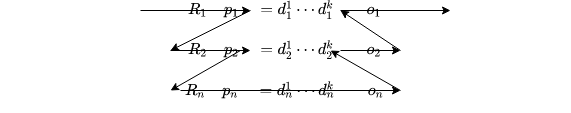
\includegraphics[width=\textwidth]{pattern.png}
\caption{Flowgraph rule evaluations}
\label{flowg}
\end{figure}
\subsection{Patterns}
\label{sec:orgc4f67ef}
\subsubsection{Variables}
\label{sec:org3f48f42}
\begin{figure}[!htb]
\begin{minipage}{0.4\textwidth}
\begin{lstlisting}
$P\llb x \rrb v =$
   x <-> v;
\end{lstlisting}
when x is first occurence
\begin{lstlisting}
$P\llb x \rrb v =$
   v != x --> l$_1$;
   v <-> copyQ;
   x <-> copyP;
   uncall copy;
   x <-> copyP;
   l$_1$ <-- v != 0;
\end{lstlisting}
\end{minipage}
\qquad
\begin{minipage}{0.4\textwidth}
\begin{lstlisting}
$\overline{P\llb x \rrb v} =$
   x <-> v;
\end{lstlisting}
when x is first occurence
\begin{lstlisting}
$\overline{P\llb x \rrb v} =$
   v != 0 --> l$_1$;
   x <-> copyP;
   call copy;
   x <-> copyP;
   v <-> copyQ;
   l$_1$ <-- v != x;
\end{lstlisting}
\end{minipage}

\caption{Semantics of variables}
\label{variables}
\end{figure}
There are two different ways a variable needs to be compiled. The most basic rule \texttt{x <-> v}, with x being the variable, will be valid whenever x first occurs in a pattern. Called in reverse, this is simply the same instruction. For every occurrence of x that is not the first occurrence, we will need to use the copy subroutine described earlier. When evaluating a variable that has occurred previously, we first need to check whether x and v are identical. This is a prerequisite for the copy subroutine to work as it results in an assertion failure in the copy subroutine; otherwise. we then switch the values into the variables that are used in the routine. We switch v into \texttt{copyQ} as this is the value that will be consumed. x will be switched into \texttt{copyP} as this is the value that will be saved. When evaluated in reverse, we check that v is 0 as this again would result in an assertion failure; we move x into \texttt{copyP} and makes a copy into \texttt{copyQ} and move it back to x and v.
\subsubsection{Constants}
\label{sec:orgffdebe5}
\begin{figure}[!htb]
\begin{minipage}{0.4\textwidth}
\begin{lstlisting}
$P \llb k \rrb v =$
    v != k --> l$_1$;
    v -= k;
    l$_1$ <-- v != 0;
\end{lstlisting}
\end{minipage}
\qquad
\begin{minipage}{0.4\textwidth}
\begin{lstlisting}
$\overline{P\llb k \rrb v} =$
    v != 0 --> l$_1$;
    v += k;
    l$_1$ <-- v != x;
\end{lstlisting}
\end{minipage}

\caption{Semantics of constants}
\label{constants}
\end{figure}
Constants are quite simple to evaluate. Firstly the constant needs to be equivalent to v for the pattern to match. We want to extract the constant k from v, getting v to equal 0 if the pattern matches. This can only be the case when they are equivalent. In the case they are, we simply subtract k from v, and since k is a constant and will never change, we cannot, and there is no need to do anything to k. In reverse, we do the opposite. We check if v is 0. If it is, we can set it to the value of k.
\subsubsection{Pairs}
\label{sec:org9a251db}
\begin{figure}[!htb]
\begin{minipage}{0.4\textwidth}
\begin{lstlisting}
$P\llb (p_1,p_2) \rrb v =$
   v & 3 --> l$_1$;
   v <-> consP;
   uncall cons;
   $t_1$ <-> consA;
   $t_2$ <-> consD;
   $P \llb p_1 \rrb t_1$;
   t$_1$ != 0 --> l$_2$;
   $P \llb p_2 \rrb t_2$;
   t$_2$ == 0 --> l$_3$;
   l$_2$ <-- t$_1$ != 0;
   $\overline{P \llb p_1 \rrb t_1}$;
   $t_1$ <-> consA;
   $t_2$ <-> consD;
   call cons;
   v <-> consP;
   l$_3$ <-- v == 0;
   l$_1$ <-- v & 3;
\end{lstlisting}
\end{minipage}
\qquad
\begin{minipage}{0.4\textwidth}
\begin{lstlisting}
$\overline{P\llb (p_1,p_2) \rrb v} =$
   v & 3 --> l$_1$;
   v == 0 -> l$_3$;
   v <-> consP;
   uncall cons;
   $t_1$ <-> consA;
   $t_2$ <-> consD;
   $P \llb p_1 \rrb t_1$;
   t$_1$ != 0 --> l$_2$;
   l$_3$ <-- t$_2$ == 0;
   $\overline{P \llb p_2 \rrb t_2}$;
   l$_2$ <-- t$_1$ != 0;
   $\overline{P \llb p_1 \rrb t_1}$;
   $t_1$ <-> consA;
   $t_2$ <-> consD;
   call cons;
   v <-> consP;
   l$_1$ <-- v & 3;
\end{lstlisting}
\end{minipage}

\caption{Semantics of pairs}
\label{pairs}
\end{figure}
When translating a pair to RIL, we first start by checking whether or not v is a pointer to a pair. This can be done by checking \texttt{v \& 3}, as pointers always will have 11 in their 2 least significant bits. If v simply is not a pair, we can skip the entire unfolding of v, jumping straight to the bottom. If v is a pair, we move v into \texttt{consP}, as we need to deconstruct by uncalling cons. the car and cdr will then be in \texttt{consA} and \texttt{consD}. It is then required to move these to two newly created variables t\textsubscript{1} and t\textsubscript{2}. This might seems unnecessary at first, but whenever we have nested patterns, not moving \texttt{consA} and \texttt{consD} out to new variables will make the program fail as these will not be 0 in the uncall to cons in the nested pair. When moved accordingly, we can then evaluate p\textsubscript{1} under t\textsubscript{1}. After this evaluation, we need to check if \texttt{v} was correctly cleared. If t\textsubscript{1} is 0, we can move on to evaluate p\textsubscript{2} under t\textsubscript{2}. Is it the case that t\textsubscript{1} is not 0, we jump to entry l\textsubscript{3} and reconstruct v\textsubscript{1}. Once again, this ensures we do not lose any information while evaluating a pattern. Then we proceed to reconstruct v by doing the inverse sequence of operations as when we deconstructed the pair. On the other hand, do we evaluate p\textsubscript{2} correctly, we can jump to entry l\textsubscript{4}. When evaluated inversely, we start by checking whether v is a pointer, skipping the entire thing if it is not. We then check whether v is 0. if it is, we jump to entry l\textsubscript{4}, and proceed to construct v by evaluating t\textsubscript{2} and t\textsubscript{1} inversely, calling cons and moving into v. If v is not 0, we have to deconstruct it even further by uncalling cons and make evaluate t\textsubscript{1}. Overall the procedure will deconstruct a pair in the forward direction and create a pair in the inverse direction.
\subsubsection{As pattern}
\label{sec:org3f92834}
\begin{figure}[!htb]
\begin{minipage}{0.4\textwidth}
\begin{lstlisting}
$P \llb x \uptext{as} (p_1,p_2) \rrb v =$
   v & 3 --> l$_1$;
   v <-> fieldsP;
   call fields;
   x <-> fieldsP;
   $t_1$ <-> fieldsA;
   $t_2$ <-> fieldsD;
   $P \llb p_1 \rrb t_1$;
   t$_1$ != 0 --> l$_2$;
   $P \llb p_2 \rrb t_2$;
   t$_2$ == 0 --> l$_3$;
   l$_2$ <-- t$_1$ != 0;
   $\overline{P \llb p_1 \rrb consA}$;
   x <-> fieldsP;
   $t_1$ <-> fieldsA;
   $t_2$ <-> fieldsD;
   uncall fields;
   v <-> fieldsP;
   l$_3$ <-- v == 0;
   l$_1$ <-- v & 3;
\end{lstlisting}
\end{minipage}
\qquad
\begin{minipage}{0.4\textwidth}
\begin{lstlisting}
$\overline{P \llb x \uptext{as} (p_1,p_2) \rrb v} =$
   v & 3 --> l$_1$;
   v == 0 -> l$_3$;
   v <-> fieldsP;
   call fields;
   x <-> fieldsP;
   $t_1$ <-> fieldsA;
   $t_2$ <-> fieldsD;
   $P \llb p_1 \rrb t_1$;
   t$_1$ != 0 --> l$_2$;
   l$_3$ <-- t$_2$ == 0;
   $\overline{P \llb p_2 \rrb t_2}$;
   l$_2$ <-- t$_1$ != 0;
   $\overline{P \llb p_1 \rrb t_1}$;
   x <-> fieldsP;
   $t_1$ <-> fieldsA;
   $t_2$ <-> fieldsD;
   uncall fields;
   v <-> fieldsP;
   l$_1$ <-- v & 3;
\end{lstlisting}
\end{minipage}

\caption{Semantics of As pattern}
\label{As}
\end{figure}
An \texttt{as} pattern is almost identical to the pairs. The only difference is that we want to keep the integrity of x, which is done by using the fields sub-routine. Just like with a pair, we check if v is, in fact, a pair. We will then move v into \texttt{fieldsP}, calling \texttt{fields} and then distributing the pointer to x, \texttt{fieldsA} to t\textsubscript{1}, and \texttt{fieldD} to t2. Again t\textsubscript{1} and t\textsubscript{2} need to be unique newly created variables, such that we do not encounter any trouble with nested patterns. The rest of the evaluation of an \texttt{as} pattern is the same as for pairs since the only difference between an \texttt{as} pattern and a \texttt{pair} pattern is that we in the \texttt{as} pattern want to keep a reference to the pair.  In reverse, the same principles also hold.
\subsubsection{Not equal (<>)}
\label{sec:orga4cfc3b}
\begin{figure}[!htb]
\begin{minipage}{0.4\textwidth}
\begin{lstlisting}
$P \llb x \neq p \rrb v =$
    assert x == 0;
    $P \llb p \rrb v$;
    x += v;
    $\overline{P \llb p \rrb v}$;
    v -= x;
\end{lstlisting}
\end{minipage}
\qquad
\begin{minipage}{0.4\textwidth}
\begin{lstlisting}
$\overline{P \llb x \neq p \rrb v} =$
    v += x;
    $P \llb p \rrb v$;
    x -= v;
    $\overline{P \llb p \rrb v}$;
    assert x == 0;
\end{lstlisting}
\end{minipage}

\caption{Semantics of <> pattern}
\label{Neq}
\end{figure}

For a \texttt{not equal} pattern, we first need to assume x is 0; otherwise, our two updates, first to x then to v, would compromise the integrity of v. For instance, in the case of flip, the rule \texttt{| x = x} could be written as \texttt{| x <> (l,r) = x <> (fr,fl)}. In such a case, v would not be a pointer (v !\& 3). Thus we skip the entire evaluation of p. we would then subtract v from x, do nothing once again, and then subtract a value larger than v from v, which is nonsensical. Therefore x must be 0 before the evaluation. As explained, after the assertion, we want to deconstruct p under v, then update x with \texttt{x += v}, setting x to v. here v should have its original value as it should skip moving v into p, else x would be equal to p. we then reconstruct p under v and subtract the value of x from v. In its core this is a simple swap, however, if p matches v, v should be 0 and no update to x is happening.

\subsection{Let definitions}
\label{secdefs}
\begin{figure}[!htb]
\begin{minipage}{0.25\textwidth}
\begin{lstlisting}
$D \llb \textup{let} p_1 = f p_2 \textup{in} \rrb =$
    $\overline{P \llb p_2 \rrb A}$;
    call f;
    $P \llb p_2 \rrb A$;
    assert A == 0;
\end{lstlisting}
\begin{lstlisting}
$D \llb \textup{let} p_1 = !f p_2 \textup{in} \rrb =$
    $\overline{P \llb p_2 \rrb A}$;
    uncall f;
    $P \llb p_2 \rrb A$;
    assert A == 0;
\end{lstlisting}
\end{minipage}
\qquad
\begin{minipage}{0.25\textwidth}
\begin{lstlisting}
$D \llb \textup{let} p_1 = \textup{loop} f p_2 \textup{in} \rrb =$
    l$_1$ <-- A != 0;
    $\overline{P \llb p_2 \rrb A}$;
    $P \llb p_1 \rrb A$;
    A == 0 --> l$_2$;
    call f;
    --> l$_1$
    l$_2$ <--
    assert x == 0;
\end{lstlisting}
\end{minipage}
\qquad\qquad
\begin{minipage}{0.30\textwidth}
\begin{lstlisting}
$D \llb \textup{let} p_1 = \textup{!loop} f p_2 \textup{in} \rrb =$
    l$_1$ <-- A != 0;
    $\overline{P \llb p_2 \rrb A}$;
    $P \llb p_1 \rrb A$;
    A == 0 --> l$_2$;
    uncall f;
    --> l$_1$
    l$_2$ <--
    assert x == 0;
\end{lstlisting}
\end{minipage}

\caption{Semantics of let definitions}
\label{defs}
\end{figure}
\subsubsection{function calls}
\label{sec:org4cc3842}
A call consists of 4 parts. First, we want to evaluate p\textsubscript{2} under A in inverse. We want to construct A from p\textsubscript{2}. This should prepare A to be the input for \texttt{f}. The call to \texttt{f} then happens, and the result is always placed in A. we then evaluate p\textsubscript{1} under A, moving the value from A into p\textsubscript{1}. Lastly, we need to assert that A is 0. this assertion is important, as it ensures that the result of \texttt{f} is a matching pattern to p\textsubscript{1}. For instance, if \texttt{f} returns 7, we cannot assign 7 to a pair; thus, such a construct should fail.
\subsubsection{Loops}
\label{sec:orgeb5df6b}
Loops are useful in situations where tail-recursive functions are needed. Nevertheless, since these are not allowed, we can write these as our loop construct. The loop will keep calling \texttt{f} until p\textsubscript{1} is matched. We first have an entry l\textsubscript{1}. This is where the loop starts. We then construct A from p\textsubscript{2}. Then right after, we deconstruct A into p\textsubscript{1}. If A is 0, it means p\textsubscript{1} was matched correctly, and we do not call the function \texttt{f} as we jump to entry l\textsubscript{2}. If A is not 0, p\textsubscript{1} is not matched, and we call the function \texttt{f}. We then jump back to l\textsubscript{1}, repeating the procedure until p\textsubscript{1} is matched.
\section{Compiler implementation}
\label{compiler}
The implementation of the evaluation functions for ARL is built on a stack of monad-transformers. The reason for choosing such a solution is that monads are a well-integrated part of Haskell, and it makes it a lot easier to implement the recursive calls to the different functions as we can use do notation to lift our functions into the monad. Furthermore, we both have an environment we want to pass on to the different \texttt{eval}-functions and some states to make it a lot easier to ensure that entries and exits are unique and that variables are correct, etc. Most importantly, the stack allows for easy extensibility as we can easily add new monad transformers to our stack. The stack looks as follows:

\begin{figure}[!htb]
\begin{lstlisting}
  type Eval a = ReaderT Env (StateT RilState Identity) a

  runEval env st ev = runIdentity $ runStateT (runReaderT ev env) st
\end{lstlisting}
\caption{The Monad stack for evaluation}
\label{stack}
\end{figure}

As can be seen from Figure\ref{stack}, the stack is fairly simple. The eval type takes an arbitrary type a; we only use \texttt{String} as this allows us to write the RIL code directly to a file. Our string is then wrapped in an identity monad. This in itself is useless but works well with other monads. This again is better for extensibility as we can always substitute for another monad such as IO, which cannot be stacked as a transformer. The identity monad is then wrapped in a state transformer, where the state itself is of the type \texttt{RilState}, which is a product type we will go over later in this section. Lastly, we wrap readerT around the State. In the future, it could be useful to add the error monad to the stack to handle failures, which we currently do not do, or the writer monad to add some logging.

\subsection{Why reader?}
\label{sec:orgf5c32eb}
The reader monad is extremely useful in our case as we have an environment we want to pass around to the different function, and it makes it easier to manage if this is not passed around as parameters but is kept isolated in the environment, which can then be locally set to the specific function calls. From section\textasciitilde{}\ref{semantics} it might be clear that we often use \texttt{A} as the variable we evaluate under, however in some cases, this change, for instance, when evaluating a pair where we need to evaluate t\textsubscript{1} and t\textsubscript{2}. Therefore we might want to keep track of this. This seems like a state, but since it never changes inside any function, we can define it in the environment. The second part of the environment is a map. We use this to keep track of which variables are alive in the program. These should be stored on the stack before a function call. This is fairly simple to do since the control flow of ARL is extremely simple. One solution might be to search the AST from the bottom up; however, since the control-flow is as simple as possible, we extract all variable IDs from a Rule into a list of ID lists. We then check if a variable in a list is in any of the following lists. If this is the case, the variable must be alive. We can then zip these results with a let declaration's unique identifier, constructing our map. Thus the Environment looks as follows:

\begin{verbatim}
   type Env = (String, M.Map String [ID])

   baseEnv = ("A", M.empty)
\end{verbatim}
\subsection{RilState}
\label{sec:orgafed8f7}
As mentioned, there is some state in RIL that we want to keep track of to make everything easier to grasp. The RilState can be seen in figure\ref{state}, where one can notice that there is quite a lot of fields for the product type. Firstly there is \texttt{ruleNo}. This simply is a counter on rules, which \texttt{rLabel} is simply the string version of \texttt{ruleNo}, so we do not have to call \texttt{show} whenever we need the rule number. This might be a bit excessive. \texttt{fnameS} will be set at the beginning of the \texttt{evalFun} and is used together with the unique identifiers for patterns and let declarations to ensure that label names do not occur multiple times. We can exploit this since we know any function name needs to be unique, and every rule needs to be unique. \texttt{LabNo} and \texttt{label} are the same duality as \texttt{ruleNo} and \texttt{rLabel} and will number jumps and entries inside the rules. Once again, to enforce no duplication of labels. It might be worth noting that the names produced this way easily become pretty obscure and a bit hard to read. \texttt{pVars} is the last field of the state. \texttt{pVars} is used to check if a variable has previously occurred in a pattern. Now that we have already gotten over how we use the reader monad, the reader might seem like a good solution for this. It would be if it were not for how pairs are evaluated. As described in section\ref{semantics}, we need to rebuild t\textsubscript{1} if it is not correctly matched, which is opposes some problems. Therefore an easier solution is to add a variable to pVars when it is first encountered, otherwise generating duplicate code, and then resetting this map back to empty right before we check \(\overline{P \llb p_1\rrb t_1\rrb}\).
\begin{figure}[!htb]
\begin{lstlisting}
data RilState = RilState { ruleNo :: Int
                         , rLabel :: String
                         , fnameS :: ID
                         , labNo :: Int
                         , label :: String
                         , pVars :: M.Map ID Int
                         }
\end{lstlisting}
\caption{The state of the RIL program}
\label{state}
\end{figure}
\subsection{Generating RIL code}
\label{sec:org57ffa3e}
Like in the parser, we have an \texttt{eval} function for each non-terminal in the AST. We use the do notation to generate the state etc., we need a specific function, and then we want to wrap the string inside the monad. We construct the strings by creating a list of strings, where each string is a RIL instruction, which then gets intercalated, with newlines to preserve structure in the RIL file. To make the code easier to read, we abstract away the operations. Functions with names v(EQ|NEQ)(0|x)(E|J) will be conditional jumps and entries, where v is equal or not to 0 or x. Plus and sub is the updates (+=) (-=) respectively. Swap is (<->). Furthermore, we have defined swap functions for each of the variables used in the 3 subroutines described in section\ref{ril} as these are used quite often, e.g., \texttt{consP x} swaps x with \texttt{consP}.

\section{Results}
\label{sec:org9631d40}
When it comes to the actual ARL compiler, it is still in its early stages. First and foremost, there are no optimizations implemented. One such optimization could be dead code removal, which would make the actual RIL file less cluttered. Furthermore, there is very little error-handling implemented in the ARL compiler itself. As described in section \ref{parsing} MegaParsec does fine error handling on its own, and we let the library handle any syntax error. We then check that functions are not defined multiple times, but the error-checking stops. This is because the compiler does not do a lot of static checks. However, the need for these checks is also minimal, when keeping in mind there are no types that need to be unified, type-checked, etc. However, one thing that is not ideal is that any errors that might occur will be RIL-errors and can be hard to identify right away. Nevertheless, error-handling is one area where the ARL compiler could improve significantly.

There are further downsides to the compiler in its current state. First and foremost, there is no adequate way to provide any program input other than lists. It means one needs to modify the RIL file to construct the desired structure in the A variable, which is highly undesirable since this a tedious and error-prone task. Despite these flaws, we successfully have implemented a compiler for ARL.

\subsection{Example Programs/tests}
\label{sec:orge22c22d}
We provide some example programs to test the evaluation and show the expressiveness of ARL.

\begin{itemize}
\item \textbf{flip}: This is the function used in the example. This program is an example of a program that needs some modification in the RIL as it is designed to work on a tree and not a list, despite it working on lists.
\item \textbf{flipN}: This function is a duplicate of flip but with the explicit disjoint patterns meaning in the \texttt{| x = x} case we specify that x cannot be equal to (l,r) as such \texttt{| x<>(l,r) = x<>(fr,fl)}. Thus this works as a test for the neq pattern.
\item \textbf{dup}: Dup is a function that duplicates a structure. This program shows that we correctly can use a variable multiple times (in a simple manner). Called in reverse, it will test that the ``forward'' direction of multiple occurrences works as well.
\item \textbf{head}: This creates a pair of the head and a list using the \texttt{as}-pattern. This program is interesting compared to the other functions we have looked at. This is because the head is an obviously non-invertible function in its classical sense. We must hereby pair it with some garbage to identify the original input. This shows some of the major limits with ARL and reversible computing in general. However, many ``regular'' functions can be expressed in ARL if we include some garbage.
\item \textbf{rev}: this shows that our loop construct works. Reverse is a fully invertible function, meaning we can use call and uncall interchangeably. We also can do this inside the loop of \texttt{reverse} which calls a helper function \texttt{rev}.
\item \textbf{abb}: This shows that copy works for more complex cases.
\end{itemize}
It should be clear that these programs show some of the interesting properties of reversible computing. One big advantage is that many functions are injective, and for partially invertible functions, we can limit ourselves only to define a function once, that can then do multiple things. An example of such would be zip and unzip functions. Clearly, these advantages hold for all reversible languages, and despite ARL's relatively low expressiveness, it has some clear advantages because of the backend. The heap manager's maximal sharing makes ARL a bit more manageable compared to RFUN etc., where one has to call a duplicate function every time a variable is used multiple times. On the other hand, ARL is still very limited in its structure. It can be difficult to make any larger programs since there is no obvious way to store results of function calls, and function calls are structured as a pipeline, which means functions in the same program must fit together. To be able to store variables would be highly valuable. Another place ARL could be improved is in the unexisting type-system. It would be very nice to be able to do arithmetic on integers etc. Lastly, since ARL is a functional language, it would make obvious sense to allow higher-order functions, potentially circumventing some of the limitations. Overall, ARL shows some great promise, and the syntax makes it quite easy to understand compared to other languages, but it is limited to do some fairly simple programs.
\section{How to use - code structure}
\label{sec:orgc069044}
The compiler is still a bit tedious to use in its current state since no good interface has been implemented. The ARL compiler will generate a RIL file, which has to be compiled by the RIL compiler, which then needs to be compiled using a C compiler. The Haskell project is built using stack and is thus required (The build details are defined in the packages.yaml file and might also work with cabal). The workflow of compiling and running an ARL file looks as follows:

\begin{verbatim}
$ stack build
$ stack exec "ARL-exe filename [options]"
\end{verbatim}
here the filename is the .arl file to compile. Notice opposite of the RIL compiler; it also needs the .arl suffix. The compiler can take some arguments, which looks as follows.
\begin{itemize}
\item -i or \texttt{-{}-input}: this is the list to provide for the build subroutine in the RIL program. This has to be an integer list. The default value is the list 1..10.
\end{itemize}
\begin{itemize}
\item -o \texttt{-{}-output}: this option specifies the name of the produced .ril file. The default option is to have the same name as the .arl file.
\item -c \texttt{-{}-compile}: This flag is a little redundant but will specify which file to compile if it is not provided.
\end{itemize}

When the RIL code has been generated, the program can be compiled to C code using the comRIL binary. We provide this in RIL-folder where it can be compiled itself\footnote{We need the entie folder as the was some weird problems with interpretation???}. Now one can compile the c file. The generated file can now be generated. If the output shows 4 lines, which shows some program statistics, the program terminated correctly. To make this project easier, we provide a Makefile to compile and run the example programs. Simply run
\begin{verbatim}
$ source makeEXc
\end{verbatim}
to compile and run all the files
To clean the repositiory run
\begin{verbatim}
$ source cleanEXc
\end{verbatim}
\subsection{Code structure}
\label{sec:org70ad947}
the project consists of the following
\begin{itemize}
\item test-folder: This folder tests the parsing both that it works correctly and fails correctly. It also tests some of the other functions used in the code. These tests could have been a lot more extensive. Lastly, the test-folder has the examples-folder. This is where all the examples files are stored.
\item RIL-folder: In this folder, the RIL compiler code is provided. This folder is not original work of the author but can be credited to Torben Ægidius Mogensen.
\item src-folder: This folder consists of the source-code to the ARL compiler. Moreover, it includes the following files:
\begin{itemize}
\item Main: Here, we do the IO, read a file, call the parser and the evaluation, and writes to a file.
\item Ast: This defines the Abstract syntax tree.
\item Parser: This file includes the parser.
\item Eval: This file defines the evaluation and the monad we evaluate under.
\item RilState: Defines the State used in the evaluation of the AST.
\item RilEnv:  Defines the Environment to read from in the evaluation.
\item RIL: specifies the general setup for the heap-manager. Such as the heap size, subroutines described in section\ref{ril} etc.
\item Util: Holds functions to make the eval-functions more manageable.
\item Options: implements the compiler options.
\end{itemize}
\end{itemize}
\section{Conclusion}
\label{sec:org08edcef}
We have in this report described the reversible functional language ARL. We have successfully reasoned about the need for a new language and its relation to the already present ones. We have given a formal overview of the language itself and presented some of the considerations taken to make the language more approachable by making the syntax so familiar to ML as possible. Likewise, we have shown some of the strict indentation rules forced upon the language to make it more readable. We have seen how the heap manager implemented in RIL can be used for ARL by following a particular compilation scheme presented by Mogensen\cite{patterns} and described in section\ref{semantics}. Using this heap manager, which uses maximal sharing, allows for features such as reuse of variables, \texttt{as}-patterns, etc. We have reasoned about how this improves the programming experience compared to popular languages in the same category, namely RFUN. However, we have omitted to make any performance comparisons of any kind. This seemed like a reasonable choice as ARL still is very limited and should not perform very well since no optimizations of any kind have been considered. We have likewise seen some of the shortcomings in ARL. These mainly relate to the ease of use and general usefulness of ARL. Currently, ARL is severely limited from the pipeline-structure, along with the limited way of specifying data structures. Furthermore, we have argued for some possible extensions that would allow ARL to be quite a bit more expressive in nature. These are features such as arithmetic, higher-order functions, etc.

\bibliographystyle{unsrt}
\bibliography{inverse}
\newpage
\begin{appendix}
\section{example-translation (flip)}
\label{appFlip}
\begin{figure}[!htb]
\begin{lstlisting}
$F\llb f\; r_1 | r_2 \rrb =$
    begin flip
    skip
    --> flip_entry_1
    flip_exit_1 <--
    skip
    end flip
$R\llb (l,r) = d_i^1, d_i^2 (fr,fl) \rrb =$
    flip_entry_1 <--
    $P\llb (l,r) \rrb A =$
        A & 3 --> l_rflip1;
        A <-> consP;
        uncall cons;
        t1l_r <-> consA;
        t2l_r <-> consD;
        l <-> t1l_r;
        t1l_r != 0 --> l_rflip2;
        r <-> t2l_r;
        t2l_r == 0 --> l_rflip3;
        l_rflip2 <-- t1l_r != 0;
        l <-> t1l_r;
        t1l_r <-> consA;
        t2l_r <-> consD;
        call cons;
        A <-> consP;
        l_rflip3 <-- A == 0;
        l_rflip1 <-- A & 3;
    A != 0 --> flip_entry_2;
    $D \llb \textup{let} fl = flip l \textup{in} \rrb =$
        $\overline{P\llb l \rrb A} =$
            l <-> A;
        r <-> M[stackP];
        stackP += 4;
        call flip;
        stackP -= 4;
        r <-> M[stackP];
        $P\llb fl \rrb A =$
            fl <-> A;
        assert A == 0;
    $D \llb \textup{let} fl = flip l \textup{in} \rrb =$
        $\overline{P\llb r \rrb A} =$
            r <-> A;
        fl <-> M[stackP];
        stackP += 4;
        call flip;
        stackP -= 4;
        fl <-> M[stackP];
        $P\llb fr \rrb A =$
            fr <-> A;
        assert A == 0;
    flip_exit_2 <-- A != 0;
\end{lstlisting}
\end{figure}
\begin{figure}[!htb]
\begin{lstlisting}
    $\overline{P\llb (fr,fl) \rrb A} =$
        A & 3 --> inv_fr_flflip8;
        A == 0 --> inv_fr_flflip10;
        A <-> consP;
        uncall cons;
        inv_t_flip8fr_fl <-> consA;
        inv_t_flip9fr_fl <-> consD;
        fr <-> inv_t_flip8fr_fl;
        inv_t_flip8fr_fl != 0 --> inv_fr_flflip9;
        inv_fr_flflip10 <-- inv_t_flip9fr_fl == 0;
        fl <-> inv_t_flip9fr_fl;
        inv_fr_flflip9 <-- inv_t_flip8fr_fl != 0;
        fr <-> inv_t_flip8fr_fl;
        inv_t_flip8fr_fl <-> consA;
        inv_t_flip9fr_fl <-> consD;
        call cons;
        A <-> consP;
        inv_fr_flflip8 <-- A & 3;
    skip
    --> flip_exit_1
$R\llb x = x \rrb =$
    flip_entry_2 <--
    $P\llb x \rrb A =$
        x <-> A;
    A != 0 --> flip_entry_3;
    flip_exit_3 <-- A != 0;
    $\overline{P\llb x \rrb A} =$
        x <-> A;
    skip
    --> flip_exit_2
flip_entry_3 <--
assert A != A
--> flip_exit_3
\end{lstlisting}
\end{figure}
\newline
\section{Parser code}
\label{appParse}
\begin{verbatim}
funP :: Parser (Either Main Func)
funP = L.nonIndented scn $ L.lineFold scn p
  where
    p sc'    = do rword "fun"
                  ind <- L.indentLevel
                  id <- identifier
                  case id of
                    "main" -> Left <$> mainP
                    _      -> Right <$> rest id ind
    rest id ind  = do r <- ruleP ind;
                      rs <- many $ try rules
                      mapM_ (\(_,x) -> when (x /= mkPos 5)
                          (L.incorrectIndent EQ (mkPos 5) x)) rs
                      return $ Func id $ r:map fst rs
    rules  = do scn
                ind <- L.indentLevel; symbol "|"
                r <- ruleP ind
                return (r,ind)
    mainP  = do symbol "="; some $ try funC
\end{verbatim}
\begin{verbatim}
defP :: Pos -> Parser Def
defP ind = try call <|> try loop <?> "Let def"
  where
      call   = do L.indentGuard scn EQ ind;
                  rword "let"
                  lhs <- patternP
                  symbol "="
                  uncall <- observing $ symbol "!"
                  fname <- identifier
                  rhs <- patternP
                  rword "in"
                  scn
                  case uncall of
                    Left _ -> return $ Call lhs fname rhs
                    Right _ -> return $ Uncall lhs fname rhs
\end{verbatim}
\begin{verbatim}
patternP :: Parser Pattern
patternP = try as <|> try neq <|> try nilnil <|>
           var <|> const' <|> try pair <|> parLE <?> "Pattern"
  where
    nilnil = rword "[[]]" >> return NilNil
    const' = (integer <|> nils) <&> Const
    nils   = rword "[]" >> return 2
    var    = identifier <&> Var
    neq    = do ident <- identifier; rword "<>"; Neq ident <$> patternP
    as     = do ident <- identifier; rword "as"; As ident <$> pair
    pair   = parens pairP
    pairP  = makeExprParser patternP
             [
                [InfixR $ Pair <$ symbol "::"],
                [InfixR $ Pair <$ symbol ","]
             ]
    parLE  = parens patternP
\end{verbatim}
\end{appendix}
\end{document}
